\documentclass[submit,techreq,noauthor]{eco}	% semi style
\usepackage[dvips]{graphicx}
\usepackage{listings, jlisting} 		% for source code
\usepackage{url}
\usepackage{setspace}
\usepackage{here}
%\setstretch{1.5} % 行間を広くします(資料チェックしてもらうときはコメントを外す)
\lstset{
  basicstyle={\ttfamily},
  identifierstyle={\small},
  commentstyle={\smallitshape},
  keywordstyle={\small\bfseries},
  ndkeywordstyle={\small},
  stringstyle={\small\ttfamily},
  frame={tb},
  breaklines=true,
  columns=[l]{fullflexible},
  numbers=left,
  xrightmargin=0zw,
  xleftmargin=3zw,
  numberstyle={\scriptsize},
  stepnumber=1,
  numbersep=1zw,
  lineskip=-0.5ex
}

\begin{document}

\semino {4/3}					% 年度/回数
\date   {4/10/28/金}				% 平成/月/日/曜日
\title  {xv6-publicにおけるブートローダの調査}	% タイトル
\author {山下 恭平}				% 氏名


\begin{abstract}
	xv6-public[1]はMITが開発したx86アーキテクチャで動作する教育用オペレーティングシステム(OS)である.xv6を動作させるにはプロセッサエミュレータQEMUを使用する.本稿ではQEMUにxv6を起動するように命令をしてから,xv6のカーネルがメモリ上に配置されるまでの一連の動作について調査を行い,BIOSとブートドライブの関係を明らかにし、ブートローダがカーネルをメモリにロードするプロセスを明らかにする.

\end{abstract}
\maketitle


\section{はじめに}
コンピュータが起動してからオペレーティングシステム(OS)が動作するまでの間に,様々なプログラム(BIOSやブートローダ)が動作している.しかし,私はOSが動作する前に動作するプログラムについての知見を持ち合わせていない.そこで,教育用OSのxv6-publicを用いてブートローダについて調査を行い,カーネルがメモリ上にロードされるまでの動作について明らかにする\\
\indent 本稿では第2章で実験環境について説明し,第3章ではxv6の起動手順を示しBIOSとブートドライブの関係を確認する,第4章では実際にブートドライブが作成される手順を確認し,第5章でブートローダの動作を明らかにし,第6章でそれらをまとめる.

\section{動作環境}
用いた実験環境について表1と図1に示す.

\begin{table}[H]
	\caption{動作環境}
	\label{table:data_type}
	\begin{tabular}{|c|c|}
		\hline
		用途                   & 名称                   \\ \hline \hline
		ホストOS               & macOS Monterey ver12.6 \\ \hline
		CPU                    & Intel Core i5-8279U    \\ \hline
		プロセッサエミュレータ & qemu-system-i386       \\ \hline
		ゲストOS               & xv6-public             \\ \hline
	\end{tabular}
\end{table}

\begin{figure}[H]
	\centering
	\includegraphics[width=5.5cm]{fig/pic1.eps}
	\caption{動作環境概略図}
	\label{sample}
\end{figure}

\section{xv6-publicの起動手順}
調査対象を明確にするためにxv6-publicの起動手順を示し,ブートドライブとBIOSの関係を確認する\\
「make qemu」コマンド実行からxv6-publicのカーネルがロードされるまでの手順は次の通りである

\begin{enumerate}
	\renewcommand{\labelenumi}{\arabic{enumi}).}
	\item BIOSが起動する
	\item qemuのオプションで指定されているブートドライブのMBR内ブートシグネチャを確認
	\item ブートシグニチャにマジックナンバーaa55が格納されているため,ブートセクタと判断しMBRをメモリの0x7c00番地へロード
	\item 0x7c00番地にロードされたブートローダが動き始める
	\item ブートローダによってカーネルがロードされる
\end{enumerate}

ここで,ブートドライブの先頭1セクタ(512byte)のことをMBR(Master Boot Record)と呼び,さらに,その末尾2byteをブートシグニチャという.ブートシグニチャにマッジクナンバー「aa55」が格納されているときに限りBIOSは指定したディスク(今回はxv6.imgというファイル)をブートドライブとして認識する仕組みが存在する.そのため,xv6.imgを設計するにあたって,組み込まなければならない条件が存在することがわかった.以下はその条件である

\begin{enumerate}
	\renewcommand{\labelenumi}{\arabic{enumi}).}
	\item xv6.imgの先頭512byteにブートローダを配置する
	\item ブートシグニチャにマジックナンバーを格納する
\end{enumerate}

次項ではこの条件に合致するxv6.imgの作成手法について確認する

\section{ブートドライブの作成}
前項で示した条件に合致するようにxv6.imgを作成しなければxv6-publicは正しく起動しない,xv6-publicでは「make」コマンドを実行すると自動的にxv6.imgが生成される.ここで,Makefileを調査することでxv6.imgの作成プロセスを明らかにしブートドライブの適切な設計手法について学ぶこととした.図2にxv6.imgを作るのに使用されているMakefile内のコマンドを示す.

\begin{figure}[H]
	\centering
	\fbox{
		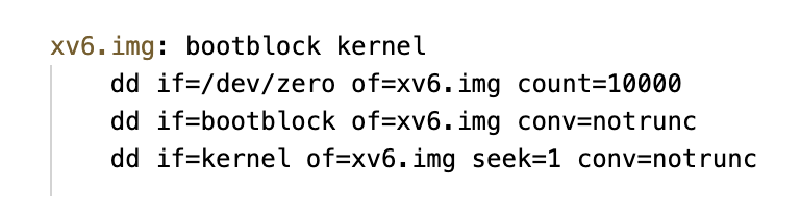
\includegraphics[scale=0.6]{fig/pic2_1.eps}
	}
	\caption{xv6.imgのMakefile}
\end{figure}

Makefile内のコマンドからxv6.imgについてわかることを以下にまとめる.

\begin{enumerate}
	\renewcommand{\labelenumi}{\arabic{enumi}).}
	\item ddコマンドによって10000ブロックの空白のファイルが生成される
	\item 先頭の1ブロックにbootblockを書き込む
	\item 2ブロック目にkernelを書き込む
\end{enumerate}

ここでddコマンドとは,ブロック単位でデータを読み書きするコマンドであり,1ブロックはデフォルトで512byteとなっている.また,seekオプションでは書き込み開始にあたってスキップするブロック数を指定する,ここではkernelの書き込みに際して「seek = 1」が指定されていることから,kernelはxv6.imgの先頭1ブロックをスキップした513byte目から書き込まれていることがわかる.図4にxv6.imgの構成イメージを示す.

\begin{figure}[H]
	\centering
	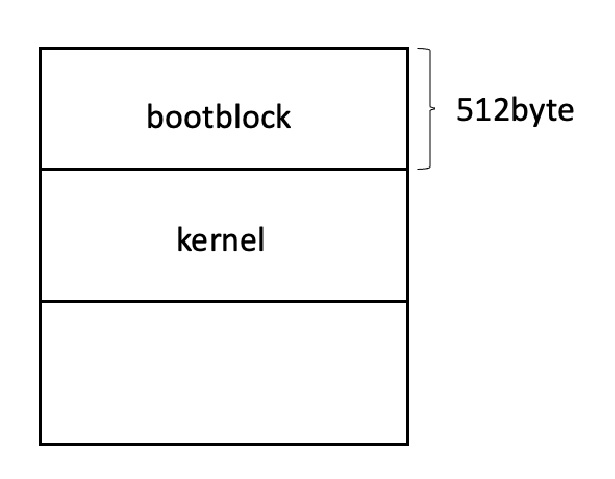
\includegraphics[width=5.5cm]{fig/pic3.eps}
	\caption{xv6.imgの構成イメージ}
	\label{sample}
\end{figure}

前項で説明したように,xv6.imgの先頭512byteにはブートローダが格納されている,従って,bootblockがブートローダ本体である.次に,bootblockを詳しく確認していく.\\
\indent 図4にbootblockを生成するMakefile内のコマンドを示す.

\begin{figure}[H]
	\centering
	\fbox{
		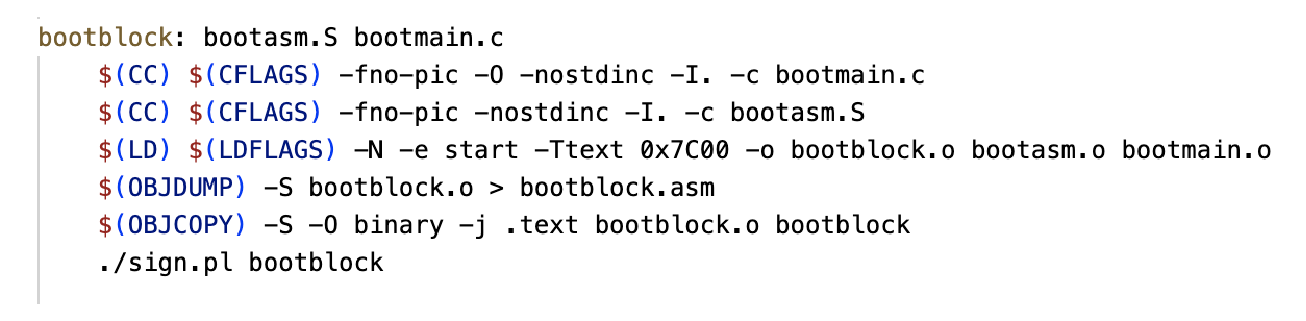
\includegraphics[scale=0.35]{fig/pic2_2.eps}
	}
	\caption{bootblockのMakefile}
	\label{sample}
\end{figure}

bootblockはbootasm.Sとbootmain.cの二つから構成されていることが確認できる.bootasm.Sとbootmain.cをそれぞれコンパイルし,生成されたオブジェクトファイルをldコマンドでリンクすることでbootblock.oを生成している.このとき「-Ttext」オプションにより開始アドレスを0x7C00番地に設定しているのがわかる,これはBIOSがブートローダを0x7C00番地へ格納することからこの地点を開始アドレスに設定していると考えられる.ここで生成されたbootblock.oをobjcopyコマンドで変換しbootblockが生成される.図5にbootblockの構成イメージを示す.

\begin{figure}[H]
	\centering
	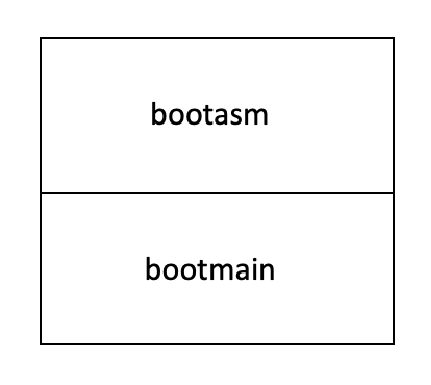
\includegraphics[width=3.5cm]{fig/pic4.eps}
	\caption{bootblockの構成イメージ}
	\label{sample}
\end{figure}

最後に,生成されたbootblockをsign.plというプログラムに読み込ませていることがわかる.そこで,sign.plのソースコード(図6)を確認すると,これはbootblockの末尾にブートシグニチャを書き込むプログラムだということが確認できた.sign.plによってxv6.imgの先頭512byteに格納されるブートローダが完成する.

\begin{figure}[H]
	\centering
	\fbox{
		\includegraphics[scale=0.4]{fig/pic5.eps}
	}
	\caption{sign.plのソースコード}
	\label{sample}
\end{figure}

ここまでの一連の流れにより,第3章で示した条件を満たすxv6.imgが生成されることが明らかとなった.次の章からは実際のブートローダの動作を確認していく.

\section{ブートローダの動作}
xv6-publicにおけるブートローダはxv6.imgに格納されているbootblockであることがわかった。この章ではブートローダの動作の詳細を明らかにすることを目的とする。\\
bootblockはbootasmとbootmainの2つのプログラムで構成されている,そのそれぞれの詳細な動作について調査を行ったが,私の理解が追いつかない部分が非常に多かったため,それぞれの動作の概略についてまとめる.

\subsection{bootasm}
bootasmは以下のことを行っていた

\begin{enumerate}
	\renewcommand{\labelenumi}{\arabic{enumi}).}
	\item 各種レジスタの初期化
	      \begin{itemize}
		      \item 図7にbootasmのアセンブリの一部を示す
		      \item \%axレジスタを0に初期化しそれを他のレジスタにコピーしている
	      \end{itemize}
	\item A20Lineの有効化
	      \begin{itemize}
		      \item x86ベースコンピュータのシステムバスを構成する電気線の1つ
	      \end{itemize}
	\item GDTの設定
	      \begin{itemize}
		      \item Global Descriptor Tableのこと
		      \item セグメントディスクリプタのセグメント管理に使用
	      \end{itemize}
	\item プロテクトモードへの移行
	      \begin{itemize}
		      \item x86アーキテクチャの動作モードの一つ
		      \item 初めはリアルモード(16bit)で動くがプロテクトモードへ移行することで32bitで動作するようになる
		      \item CR0レジスタ(図8[1])の0bit目を1にすることで移行できる
	      \end{itemize}
	\item bootmainの呼び出し
\end{enumerate}

\begin{figure}[H]
	\centering
	\fbox{
		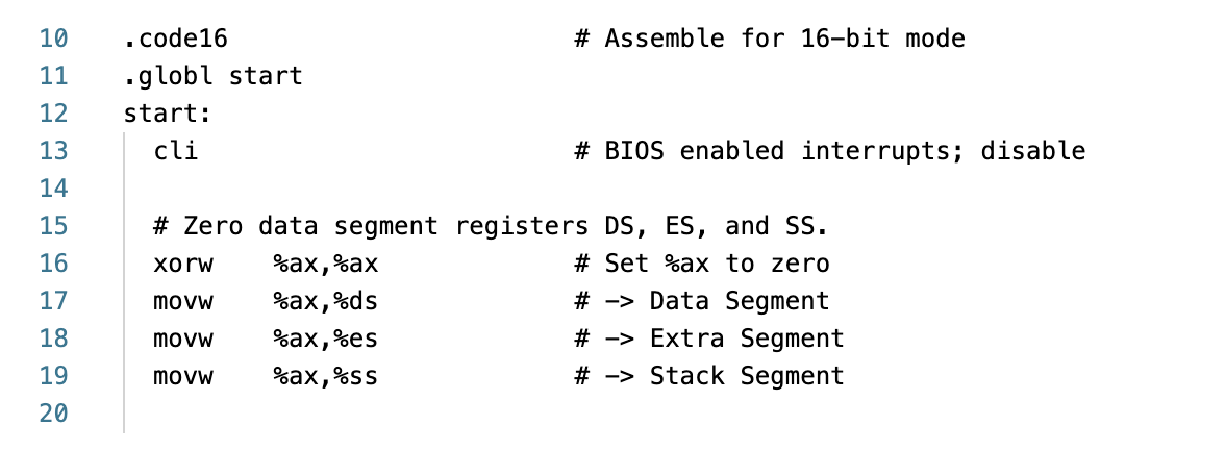
\includegraphics[scale=0.4]{fig/pic7.eps}
	}
	\caption{各レジスタの初期化}
	\label{sample}
\end{figure}

\begin{figure}[H]
	\centering
	\fbox{
		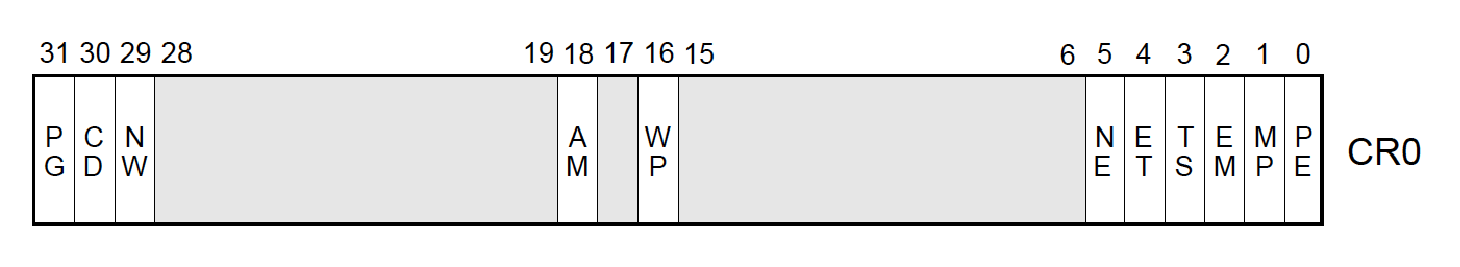
\includegraphics[scale=0.3]{fig/pic6.eps}
	}
	\caption{コントロールレジスタ0}
	\label{sample}
\end{figure}

\subsection{bootmain}
\begin{enumerate}
	\renewcommand{\labelenumi}{\arabic{enumi}).}
	\item xv6.imgの2セクタ目をロード
	      \begin{itemize}
		      \item ソースコード28行目(図9)
	      \end{itemize}
	\item elfヘッダを持つか確認
	      \begin{itemize}
		      \item ソースコード31行目
	      \end{itemize}
	\item programヘッダから情報を取得しカーネルをロード
	      \begin{itemize}
		      \item  ソースコード35行目から42行目
	      \end{itemize}
	\item entry()の呼び出し
	      \begin{itemize}
		      \item ソースコード47行目
	      \end{itemize}
\end{enumerate}

bootmainはカーネルをメモリ上にロードすることを目的としたプログラムである.
28行目で取得したプログラムヘッダの情報をもとに39行目でreadseg()関数を呼び出すことで,カーネルをメモリにロードしている.ここでreadseg関数は第1引数にロード先,第2引数にロードするデータサイズ,第3引数にxv6.imgの2ブロック目からのオフセットを入力する.つまり,28行目のreadsegでは変数elfに,xv6.imgの2セクタ目の先頭から,4096byte分の情報をロードしている.このときxv6.imgの2セクタ目にはkernelが格納されている.図10はプログラムヘッダの内容をobjdumpコマンドにより表示させた物である.ここに格納されている情報が39行目のreadseg()の引数として使用されることで,メモリ上にカーネルがロードされる.
\begin{figure}[H]
	\centering
	\fbox{
		\includegraphics[scale=0.4]{fig/pic8.eps}
	}
	\caption{bootmain.c}
	\label{sample}
\end{figure}

\begin{figure}[H]
	\centering
	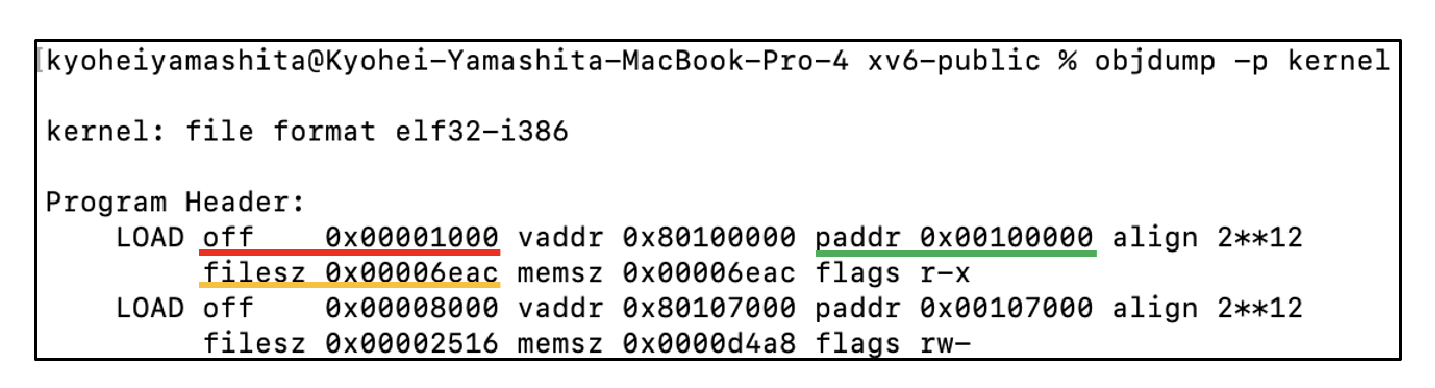
\includegraphics[scale=0.4]{fig/pic9.eps}
	\caption{プログラムヘッダの情報}
	\label{sample}
\end{figure}

\section{おわりに}
xv6-publicが起動してからカーネルがロードされるまでの動作について,ブートドライブの構成から明らかにすることで理解を深めることができた.ブートドライブとブートローダの設計には,OSについての知識だけでなくBIOSやx86アーキテクチャなど低階層における知識を体系的に取得している必要があることを知ることができた.そのため,本稿の後半部分に当たる,実際にブートローダの動作を確認を行う調査が私の知識不足より,浅い理解しかできず,資料の作成にとても戸惑ってしまった.今後は,私自身の知識の補完を行ってから再び調査を行うことや,BIOSではなくUEFIについての調査も行っていきたい.


% 参考文献はここに記述
\begin{thebibliography}{99}
	\bibitem{xv6}mit-pods/xv6-public
	\textless\url{https://github.com/mit-pdos/xv6-public}
	\textgreater (accessed 2022-10-30).
	\bibitem{intel}Intel 64 and IA-32 Architectures Software Developer’s Manual, Volume 3A: System Programming Guide, Part 1, P74
	\textless\url{https://www.intel.co.jp/content/www/jp/ja/architecture-and-technology/64-ia-32-architectures-software-developer-vol-3a-part-1-manual.html}
	\textgreater (accessed 2022-10-30).
\end{thebibliography}


\end{document}
